\section{Nhận diện chữ số trên thẻ Mastercard}

\subsection{Đề bài}
Nhận dạng chữ số trên thẻ tín dụng Mastercard
\begin{center}
    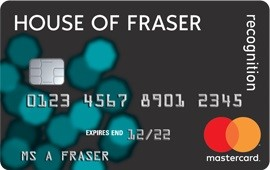
\includegraphics[scale = 1.2]{images/mastercard/inputMastercard}
\end{center}
\begin{figure}[h]
    \caption{Thẻ tín dụng Mastercard}
\end{figure}

\subsection{Mô hình nhận dạng}

    \quad Vì thẻ Mastercard có ký tự chữ số khác với chữ số thường nên ta sẽ thực
hiện training với tập dữ liệu riêng.

    \quad Ta lên mạng gõ tìm font chữ của thẻ mastercard sau đó cài đặt, vào word
gõ 100 ký tự số từ 0 đến 1 và chụp màng hình. 

    \quad Dữ liệu training là ảnh dưới đây.
\begin{center}
    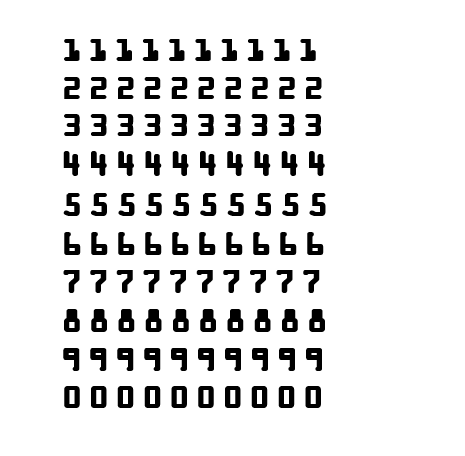
\includegraphics[scale = 1.2]{images/mastercard/training.png}
\end{center}
\begin{figure}[htp]
    \caption{ảnh training Mastercard}
\end{figure}



\tikzset{every picture/.style={line width=0.75pt}} %set default line width to 0.75pt        
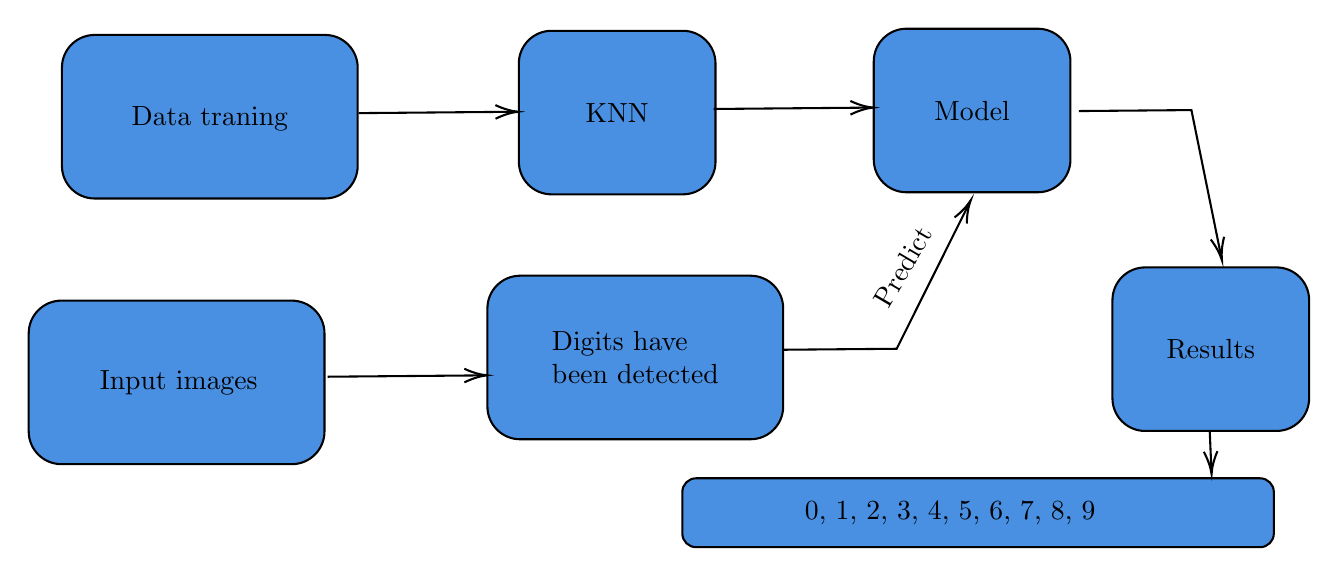
\begin{tikzpicture}[x=0.75pt,y=0.75pt,yscale=-1,xscale=1]

%uncomment if require: \path (0,300); %set diagram left start at 0, and has height of 300

%Rounded Rect [id:dp8637321097847608] 
\draw  [fill={rgb, 255:red, 74; green, 144; blue, 226 }  ,fill opacity=1 ] (45,58.96) .. controls (45,50.26) and (52.06,43.2) .. (60.76,43.2) -- (171.74,43.2) .. controls (180.44,43.2) and (187.5,50.26) .. (187.5,58.96) -- (187.5,106.24) .. controls (187.5,114.94) and (180.44,122) .. (171.74,122) -- (60.76,122) .. controls (52.06,122) and (45,114.94) .. (45,106.24) -- cycle ;
%Rounded Rect [id:dp5410094852287093] 
\draw  [fill={rgb, 255:red, 74; green, 144; blue, 226 }  ,fill opacity=1 ] (265.14,56.96) .. controls (265.14,48.26) and (272.19,41.2) .. (280.9,41.2) -- (344.14,41.2) .. controls (352.84,41.2) and (359.9,48.26) .. (359.9,56.96) -- (359.9,104.24) .. controls (359.9,112.94) and (352.84,120) .. (344.14,120) -- (280.9,120) .. controls (272.19,120) and (265.14,112.94) .. (265.14,104.24) -- cycle ;
%Straight Lines [id:da9760767594548312] 
\draw    (188,80.87) -- (242.19,80.4) -- (262.81,80.22) ;
\draw [shift={(264.81,80.2)}, rotate = 539.5] [color={rgb, 255:red, 0; green, 0; blue, 0 }  ][line width=0.75]    (10.93,-3.29) .. controls (6.95,-1.4) and (3.31,-0.3) .. (0,0) .. controls (3.31,0.3) and (6.95,1.4) .. (10.93,3.29)   ;

%Rounded Rect [id:dp7471055828977062] 
\draw  [fill={rgb, 255:red, 74; green, 144; blue, 226 }  ,fill opacity=1 ] (436.14,55.96) .. controls (436.14,47.26) and (443.19,40.2) .. (451.9,40.2) -- (515.14,40.2) .. controls (523.84,40.2) and (530.9,47.26) .. (530.9,55.96) -- (530.9,103.24) .. controls (530.9,111.94) and (523.84,119) .. (515.14,119) -- (451.9,119) .. controls (443.19,119) and (436.14,111.94) .. (436.14,103.24) -- cycle ;
%Straight Lines [id:da5013878291768636] 
\draw    (359,78.87) -- (413.19,78.4) -- (433.81,78.22) ;
\draw [shift={(435.81,78.2)}, rotate = 539.5] [color={rgb, 255:red, 0; green, 0; blue, 0 }  ][line width=0.75]    (10.93,-3.29) .. controls (6.95,-1.4) and (3.31,-0.3) .. (0,0) .. controls (3.31,0.3) and (6.95,1.4) .. (10.93,3.29)   ;

%Rounded Rect [id:dp6528048454804998] 
\draw  [fill={rgb, 255:red, 74; green, 144; blue, 226 }  ,fill opacity=1 ] (250,174.96) .. controls (250,166.26) and (257.06,159.2) .. (265.76,159.2) -- (376.74,159.2) .. controls (385.44,159.2) and (392.5,166.26) .. (392.5,174.96) -- (392.5,222.24) .. controls (392.5,230.94) and (385.44,238) .. (376.74,238) -- (265.76,238) .. controls (257.06,238) and (250,230.94) .. (250,222.24) -- cycle ;
%Straight Lines [id:da12787707134989956] 
\draw    (393,194.87) -- (447.19,194.4) -- (482.01,124.59) ;
\draw [shift={(482.9,122.8)}, rotate = 476.51] [color={rgb, 255:red, 0; green, 0; blue, 0 }  ][line width=0.75]    (10.93,-3.29) .. controls (6.95,-1.4) and (3.31,-0.3) .. (0,0) .. controls (3.31,0.3) and (6.95,1.4) .. (10.93,3.29)   ;

%Rounded Rect [id:dp8038417418505817] 
\draw  [fill={rgb, 255:red, 74; green, 144; blue, 226 }  ,fill opacity=1 ] (29,186.96) .. controls (29,178.26) and (36.06,171.2) .. (44.76,171.2) -- (155.74,171.2) .. controls (164.44,171.2) and (171.5,178.26) .. (171.5,186.96) -- (171.5,234.24) .. controls (171.5,242.94) and (164.44,250) .. (155.74,250) -- (44.76,250) .. controls (36.06,250) and (29,242.94) .. (29,234.24) -- cycle ;
%Straight Lines [id:da928144777217258] 
\draw    (173,207.87) -- (227.19,207.4) -- (247.81,207.22) ;
\draw [shift={(249.81,207.2)}, rotate = 539.5] [color={rgb, 255:red, 0; green, 0; blue, 0 }  ][line width=0.75]    (10.93,-3.29) .. controls (6.95,-1.4) and (3.31,-0.3) .. (0,0) .. controls (3.31,0.3) and (6.95,1.4) .. (10.93,3.29)   ;

%Rounded Rect [id:dp5430112256925095] 
\draw  [fill={rgb, 255:red, 74; green, 144; blue, 226 }  ,fill opacity=1 ] (551.14,170.96) .. controls (551.14,162.26) and (558.19,155.2) .. (566.9,155.2) -- (630.14,155.2) .. controls (638.84,155.2) and (645.9,162.26) .. (645.9,170.96) -- (645.9,218.24) .. controls (645.9,226.94) and (638.84,234) .. (630.14,234) -- (566.9,234) .. controls (558.19,234) and (551.14,226.94) .. (551.14,218.24) -- cycle ;
%Straight Lines [id:da1692659209791012] 
\draw    (535,79.87) -- (589.19,79.4) -- (603.5,149.84) ;
\draw [shift={(603.9,151.8)}, rotate = 258.52] [color={rgb, 255:red, 0; green, 0; blue, 0 }  ][line width=0.75]    (10.93,-3.29) .. controls (6.95,-1.4) and (3.31,-0.3) .. (0,0) .. controls (3.31,0.3) and (6.95,1.4) .. (10.93,3.29)   ;

%Rounded Rect [id:dp017160020304928025] 
\draw  [fill={rgb, 255:red, 74; green, 144; blue, 226 }  ,fill opacity=1 ] (343.9,263.44) .. controls (343.9,259.77) and (346.87,256.8) .. (350.54,256.8) -- (622.26,256.8) .. controls (625.93,256.8) and (628.9,259.77) .. (628.9,263.44) -- (628.9,283.36) .. controls (628.9,287.03) and (625.93,290) .. (622.26,290) -- (350.54,290) .. controls (346.87,290) and (343.9,287.03) .. (343.9,283.36) -- cycle ;
%Straight Lines [id:da025021326632976626] 
\draw    (598,233.8) -- (598.81,252.8) ;
\draw [shift={(598.9,254.8)}, rotate = 267.55] [color={rgb, 255:red, 0; green, 0; blue, 0 }  ][line width=0.75]    (10.93,-3.29) .. controls (6.95,-1.4) and (3.31,-0.3) .. (0,0) .. controls (3.31,0.3) and (6.95,1.4) .. (10.93,3.29)   ;


% Text Node
\draw (116.25,83.6) node  [align=left] {Data traning};
% Text Node
\draw (312.52,80.6) node  [align=left] {KNN};
% Text Node
\draw (483.52,79.6) node  [align=left] {Model};
% Text Node
\draw (321.25,198.6) node  [align=left] {Digits have \\been detected};
% Text Node
\draw (101.25,210.6) node  [align=left] {Input images};
% Text Node
\draw (450,154.8) node [rotate=-300.5] [align=left] {Predict};
% Text Node
\draw (598.52,194.6) node  [align=left] {Results};
% Text Node
\draw (473,273.8) node  [align=left] {0, 1, 2, 3, 4, 5, 6, 7, 8, 9};

\end{tikzpicture}

\begin{figure}[htp]
    \caption{Lưu đồ nhận dạng chữ số trên thẻ Mastercard}
\end{figure}


\subsection{Chương trình nhận dạng}
\begin{lstlisting}[language=Python, caption=Recognition Mastercard]
import numpy as np
#from scipy.misc.pilutil import imresize
import cv2 
from skimage.feature import hog
from matplotlib import pyplot as plot
from sklearn.model_selection import train_test_split
from sklearn.metrics import accuracy_score
from sklearn.utils import shuffle
from sklearn import datasets
from skimage import exposure
import imutils
from imutils import contours

#Khai bao ham xu li pixel de nhan dang
def pixels_to_hog_20(img_array):
    hog_featuresData = []
    for img in img_array:
        fd = hog(img, 
                 orientations=10, 
                 pixels_per_cell=(5,5),
                 cells_per_block=(1,1), 
                 visualize=False)
        hog_featuresData.append(fd)
    hog_features = np.array(hog_featuresData, 'float64')
    return np.float32(hog_features)

#Tao class KNN_MODEL
class KNN_MODEL():
    def __init__(self, k = 3):
        self.k = k
        self.model = cv2.ml.KNearest_create()

    def train(self, samples, responses):
        self.model.train(samples, cv2.ml.ROW_SAMPLE, responses)

    def predict(self, samples):
        retval, results, neigh_resp, dists = self.model.findNearest(samples, self.k)
        return results.ravel()
    
#Khai bao ham xu li anh, nhan dang anh
out_image = {}
def proc_user_img(img_file, model):
    print('loading "%s for digit recognition" ...' % img_file)
    im = cv2.imread(img_file)  
    im = imutils.resize(im,width=300)  
    imgray = cv2.cvtColor(im,cv2.COLOR_BGR2GRAY)
    rectKernel = cv2.getStructuringElement(cv2.MORPH_RECT, (9, 3))
    sqKernel = cv2.getStructuringElement(cv2.MORPH_RECT, (5, 5))
    tophat = cv2.morphologyEx(imgray, cv2.MORPH_TOPHAT, rectKernel)
    gradX = cv2.Sobel(tophat, ddepth=cv2.CV_32F, dx=1, dy=0,ksize=-1)
    gradX = np.absolute(gradX)
    (minVal, maxVal) = (np.min(gradX), np.max(gradX))
    gradX = (255 * ((gradX - minVal) / (maxVal - minVal)))
    gradX = gradX.astype("uint8")
    gradX = cv2.morphologyEx(gradX, cv2.MORPH_CLOSE, rectKernel)
    
    thresh = cv2.threshold(gradX, 0, 255,cv2.THRESH_BINARY | cv2.THRESH_OTSU)[1]
    thresh = cv2.morphologyEx(thresh, cv2.MORPH_CLOSE, sqKernel)

    #Phat giac duong bien de dong khung 
    _,contours,hierarchy = cv2.findContours(thresh.copy(), cv2.RETR_EXTERNAL, cv2.CHAIN_APPROX_SIMPLE)
    locs = []

    #Loai bo cac vung de chon duoc 4 vung anh co 4 so tren ma the
    for i,c in enumerate(contours):
        (x,y,w,h) = cv2.boundingRect(c)
        ar = w/float(h)

        if ar > 2.5 and ar < 4.0:
            if (w > 40 and w < 55) and (h > 13 and h < 20):
                locs.append((x, y, w, h))

    locs = sorted(locs, key=lambda x:x[0])
    output = [] 
    #Dua vao toa do duong bien cac vung ta thuc hien nhan dang tung vung
    j = 1 #Bien dem vong for
    for i, (gX, gY, gW, gH) in enumerate(locs):
        k = 0 #Bien dem vong for nho tu 0 - 3
        groupOutput = [] 
        group = imgray[gY - 3:gY + gH + 3, gX - 3:gX + gW + 3]
        group = cv2.threshold(group, 0, 255,cv2.THRESH_BINARY | cv2.THRESH_OTSU)[1]
        _,contours,hierarchy = cv2.findContours(group.copy(), cv2.RETR_EXTERNAL,cv2.CHAIN_APPROX_SIMPLE)

        #Thuc hien nhan dang tung anh
        for i,c in enumerate(contours):
            (x,y,w,h) = cv2.boundingRect(c)

            im_digit = group[y-1:y+h+1,x-1:x+w+1]
            im_digit = (255-im_digit)
            im_digit = cv2.resize(im_digit,(57,88))
            hog_img_data = pixels_to_hog_20([im_digit])
            
            kq = model.predict(hog_img_data)
            string = str(int(kq[0]))
            groupOutput.append(string)

            out_image[str(j*4 -1 - k)] = im_digit
            k = k +1
            
        j = j +1
        #Ghi ket qua len cac anh do 
        cv2.rectangle(im,(gX - 5, gY - 5),(gX + gW + 5, gY + gH + 5), (255, 0, 255), 2)
        cv2.putText(im, "".join(groupOutput[::-1]), (gX, gY - 15),cv2.FONT_HERSHEY_SIMPLEX, 0.65, (0, 0, 255), 2)
        output.extend(groupOutput)
       
    return im      

#Khai bao ham lay so tu anh tham chieu (reference)
def get_digits(contours, hierarchy):
    hierarchy = hierarchy[0]
    bounding_rectangles = [cv2.boundingRect(ctr) for ctr in contours]   
    final_bounding_rectangles = []
    u, indices = np.unique(hierarchy[:,-1], return_inverse=True)
    most_common_heirarchy = u[np.argmax(np.bincount(indices))]
    for r,hr in zip(bounding_rectangles, hierarchy):
        x,y,w,h = r
        if ((w*h)>250) and (10 <= w <= 200) and (10 <= h <= 200) and hr[3] == most_common_heirarchy: 
            final_bounding_rectangles.append(r)    
    return final_bounding_rectangles

#Khai bao ham sap xep ccacso tham chieu trong anh va danh so thu tu
def get_contour_precedence(contour, cols):
    return contour[1] * cols + contour[0]

#Khai bao ham load anh tham chieu va xu li
def load_digits_custom(img_file):
    train_data = []
    train_target = []
    start_class = 1
    im = cv2.imread(img_file)
    imgray = cv2.cvtColor(im,cv2.COLOR_BGR2GRAY)
    thresh = cv2.threshold(imgray,11,255,cv2.THRESH_BINARY_INV)[1]   
       
    _,contours,hierarchy = cv2.findContours(thresh.copy(), cv2.RETR_EXTERNAL, cv2.CHAIN_APPROX_SIMPLE)
    digits_rectangles = get_digits(contours,hierarchy)  
    digits_rectangles.sort(key=lambda x:get_contour_precedence(x, im.shape[1]))
     
    for index,rect in enumerate(digits_rectangles):
        x,y,w,h = rect
        cv2.rectangle(im,(x-8,y-8),(x+w+8,y+h+8),(0,255,0),2)
        im_digit = thresh[y:y+h,x:x+w]
        im_digit = (255-im_digit)
        
        im_digit = cv2.resize(im_digit,(57,88))
        train_data.append(im_digit)
        train_target.append(start_class%10)

        if index>0 and (index+1) % 10 == 0:
            start_class += 1
    
    return np.array(train_data), np.array(train_target)

#------------------chuan bi du lieu------------------
#Anh tham chieu va anh nhan dang
TRAIN_IMG = 'images\ocr-reference-1.png'
DETECT_IMG = 'images\mastercard.png'

digits, labels = load_digits_custom(TRAIN_IMG)

#In thong tin anh tham chieu
print('train data shape',digits.shape)
print('test data shape',labels.shape)

#Thuc hien sap xep ngau nhien va chuan bi du lieu de training
digits, labels = shuffle(digits, labels, random_state=256)  #Xao tron du lieu
train_digits_data = pixels_to_hog_20(digits)
X_train, X_test, y_train, y_test = train_test_split(train_digits_data, labels, test_size=0.7)

#------------------training va nhan dang anh------------------

#Thuc hien training va in ket qua % do chinh xac
model = KNN_MODEL(k = 5)
model.train(X_train, y_train)
preds = model.predict(X_test)
print('Accuracy: ',accuracy_score(y_test, preds))

#Thuc hien nhan dang anh 
model = KNN_MODEL(k = 5)
model.train(train_digits_data, labels)
im = proc_user_img(DETECT_IMG, model)

#------------------xuat ket qua------------------

#Xuat ket qua ra dang anh va imshow
cv2.imwrite("results\Ket_qua_mastercard.png",im)
cv2.namedWindow("Ket_qua_mastercard",cv2.WINDOW_AUTOSIZE)
cv2.imshow("Ket_qua_mastercard", im)

#Xuat tung so truoc khi nhan dang ra plot show
titles = {}
photo = {}
for so in range(0,16):		
    titles[str(so)] = str(so)
    photo[str(so)] = out_image[str(so)]

for i in range(0,16):
	plot.subplot(4,4,i+1), plot.imshow(photo[str(i)],'gray')
	plot.title(titles[str(i)])
	plot.xticks([]), plot.yticks([])
plot.show()
    
cv2.waitKey() 
cv2.destroyAllWindows()          


\end{lstlisting}

\subsection{Đánh giá kết quả và kết luận}

- Đầu tiên ta load hai ảnh gồm ảnh tham chiếu và ảnh thẻ tín dụng
\begin{lstlisting}[language=Python]
    #Anh tham chieu va anh nhan dang
    TRAIN_IMG = 'images\ocr-reference-1.png'
    DETECT_IMG = 'images\mastercard.png'
    digits, labels = load_digits_custom(TRAIN_IMG)
\end{lstlisting}

- Hàm load\_digits\_custom để xử lí cắt 100 số trong ảnh tham chiếu ra và thực hiện xử lí nó thành mảng các số

- Sau đó ta test nó bằng các xáo trộn dữ liệu, thực hiện xử lí và đưa ra phần trăm chính xác

\begin{lstlisting}[language=Python]
    #Thuc hien sap xep ngau nhien va chuan bi du lieu de training
    digits, labels = shuffle(digits, labels, random_state=256)  #Xao tron du lieu
    train_digits_data = pixels_to_hog_20(digits)
    X_train, X_test, y_train, y_test = train_test_split(train_digits_data, labels, test_size=0.7)

    #------------------training va nhan dang anh----------------
    #Thuc hien training va in ket qua % do chinh xac
    model = KNN_MODEL(k = 5)
    model.train(X_train, y_train)
    preds = model.predict(X_test)
    print('Accuracy: ',accuracy_score(y_test, preds))
\end{lstlisting}

- Sau đó thực hiện nhận dạng ảnh
\begin{lstlisting}[language=Python]
    #Thuc hien nhan dang anh 
    model = KNN_MODEL(k = 5)
    model.train(train_digits_data, labels)
    im = proc_user_img(DETECT_IMG, model)
\end{lstlisting}

- Hàm proc\_user\_img() để tiền xử lí ảnh nhận dạng và nhận dạng nó

- Sau khi nhận dạng xong ta thực hiện imshow từng số trước nhận dạng và kết quả, đồng thời cũng xuất ảnh kết quả ra file .png
\begin{lstlisting}[language=Python]
    #Xuat ket qua ra dang anh va imshow
    cv2.imwrite("results\Ket_qua_mastercard.png",im)
    cv2.namedWindow("Ket_qua_mastercard",cv2.WINDOW_AUTOSIZE)
    cv2.imshow("Ket_qua_mastercard", im)

    #Xuat tung so truoc khi nhan dang ra plot show
    titles = {}
    photo = {}
    for so in range(0,16):		
        titles[str(so)] = str(so)
        photo[str(so)] = out_image[str(so)]

    for i in range(0,16):
	    plot.subplot(4,4,i+1), plot.imshow(photo[str(i)],'gray')
	    plot.title(titles[str(i)])
	    plot.xticks([]), plot.yticks([])
    plot.show()
    
    cv2.waitKey() 
    cv2.destroyAllWindows()          
\end{lstlisting}

\quad \textbf{KẾT QUẢ NHẬN ĐƯỢC} \\[0.2cm]

- Các chử số trên thẻ sau khi được detect 

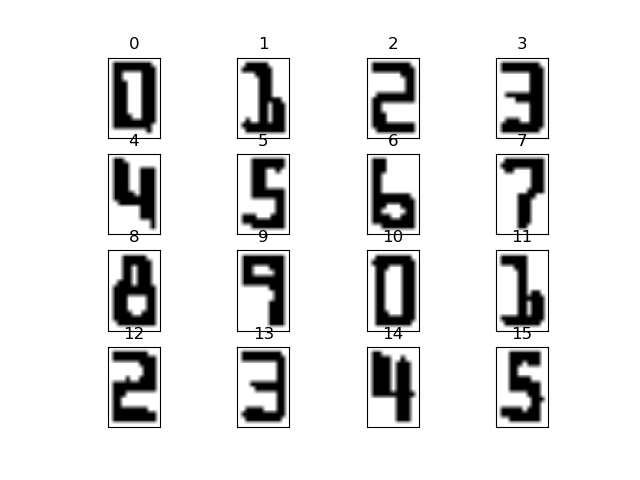
\includegraphics[]{images/mastercard/digits.png}

\begin{figure}[htp!]
    \caption{Các chử số sau khi phát hiện trên thẻ Mastercard}
\end{figure}

- Kết quả cuối cùng sau khi nhận dạng thẻ Mastercard
\begin{center}
    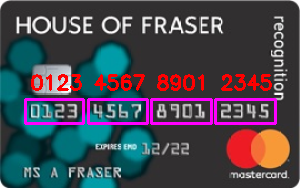
\includegraphics[]{images/mastercard/Ket_qua_mastercard.png}
\end{center}

\begin{figure}[htp!]
    \caption{Kết quả sau khi nhận dạng Mastercard}
\end{figure}